\subsection{実装量}
図~\ref{fig:hardware}に示した各モジュールを実装した結果、それぞれのVerilog実装量は表~\ref{tab:sourcesize}のようになった。
\begin{table}[h]
    \begin{center}
        \caption{各モジュールのVerilog実装量}\label{tab:sourcesize}
        \begin{tabular}{|l|l|l|}
            \hline
            ファイル名                   & 機能                                                                                       & 実装量         \\ \hline\hline
            TSPTop.v   / TSPTop\_wrap.sv & トップモジュール                                                                                 & 40行 +   57行 \\\hline
            Tsp.sv                       & \begin{tabular}[c]{@{}l@{}}・グラフ情報の管理\\・各交換モジュールの呼び出し\\・頂点スワップの実行\end{tabular} & 249行        \\\hline
            Swap.sv                      & 非隣接点交換モジュール                                                                              & 95行         \\\hline
            Swap\_adjacent.sv            & 隣接点交換モジュール                                                                               & 82行         \\\hline
            Graph.sv                     & グラフ生成モジュール                                                                               & 43行         \\\hline
            Distance.v                   & 距離計算モジュール                                                                                & 37行         \\\hline
            Xorshift.v                   & 乱数生成モジュール                                                                                & 25行         \\\hline
            Seg7.sv                      & 7セグ16進出力モジュール                                                                            & 32行         \\\hline\hline
            合計                         &                                                                                          & 約660行      \\\hline
            \end{tabular}
    \end{center}
\end{table}
\subsection{シミュレーション結果}
PC上でテストベンチを実行し、シミュレーション結果を得た。
シミュレーション結果を図~\ref{fig:sim}に示す。
\begin{figure}[h]
    \begin{center}
        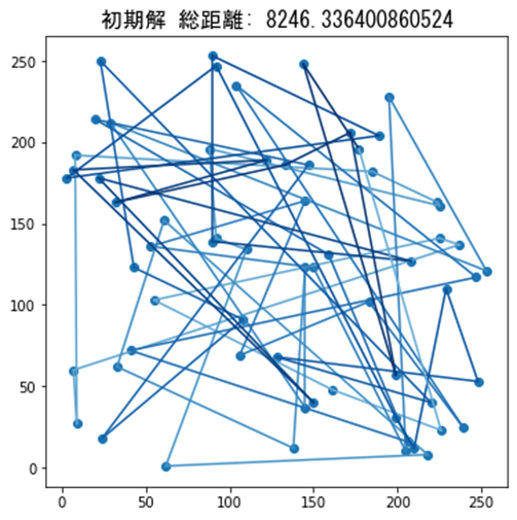
\includegraphics[width=7cm]{figure/fpga_tsp_bad.png}
        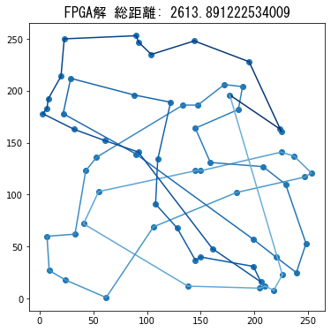
\includegraphics[width=7cm]{figure/fpga_tsp_good.png}
        \caption{シミュレーション結果}\label{fig:sim}
    \end{center}
\end{figure}
リセット入力を与えると、左図のようにランダムなグラフ・経路が生成される。
その後、右図のように山登り法によって経路が更新されていく。最終的には右図のように局所最適解に陥り、今回定めた近傍(パターン1・パターン2)だけではこれ以上改善しない状態になった。

乱数的な手法を用いているため、実行するたびに結果が異なるが、総距離2600~2800程度の局所最適解に陥ることが多かった。
並列度ごとに、局所最適解に陥るまでに要するクロック数を計測した結果を表~\ref{tab:time}に示す。
\begin{table}[h]
    \begin{center}
        \caption{並列度ごとの局所最適解に陥るまでに要するクロック数}\label{tab:time}
        \begin{tabular}{|c|c|}
            \hline
            並列度 & 局所最適解に陥るまでに要するクロック数 \\ \hline
            1      & 19.4kクロック                     \\ \hline
            2      & 11.3kクロック                       \\ \hline
            3      & 6.5kクロック                       \\ \hline
        \end{tabular}
    \end{center}
\end{table}
並列度を$n$にすると、局所最適解に陥るまでに要するクロック数は$\frac{1}{n}$になると予想されるが、概ねその通りの結果となった。
\subsection{合成結果}\label{sec:compile}
Quartus上でコンパイルを行い、並列度ごとに最大周波数・使用ロジック数・使用演算器数を計測した結果を表~\ref{tab:compile}に示す。
\begin{table}[h]
    \begin{center}
        \caption{並列度ごとの合成結果}\label{tab:compile}
        \begin{tabular}{|c|c|c|c|}
            \hline
            並列度(パターン1 + パターン2) & 最大周波数 & 使用ロジック数 & 使用演算器数 \\ \hline
            1+0      & 12.76MHz    &  7,470          & 8       \\ \hline
            0+1      & 12.69MHz    &  6,743          & 8       \\ \hline
            1+1      & 12.83MHz    & 14,821          & 16       \\ \hline
            2+1      & 12.73MHz    & 23,152          & 24       \\ \hline
            3+1      & ×(合成失敗)        & 50,546          & 32       \\ \hline
        \end{tabular}
    \end{center}
\end{table}

並列度を上げても最大周波数はほとんど変化しなかった。
使用ロジック数は、pow(2, 総並列度)に比例して指数関数的に増加した。並列度4では、使用ロジック数がFPGAのリソースを超えてしまったため、合成に失敗した。
使用演算器数は、総並列度に線形に増加した。各交換モジュールあたり8個の演算器を必要としていて、これらは距離計算モジュールに割り当てられていた。

使用ロジックの内訳として、各交換モジュールは4000程度(うち距離計算が2000程度)しかなく、これらのモジュールを並列につなぎ合わせる部分が使用ロジック数の大きく占めることがわかった。